The SSP1-MOB vision of the future described in \sref{s:results:ssp1-mob} is used in the following sections to synthesise the changes that the mobility paradigm must undergo\footnote{The changes are not ``suffered'' by an autonomous and disconnected system of mobility, but are introduced by all the agents that play a part in it: users, industries, governments, decision makers, researchers, planners, etc.} to reach the desired form. The synthesis is done using backcasting approach, for which an ``intermediate step'' is presented in \ssref{ss:results:backcasting-2050-intermediate-step}. This halfway step is described in terms of the same variables highlighted in \tref{t:ssp1-mob-2100-narrative-thesis}, but adding information for the year 2050. The baseline ``scenario'' status of 2017 is also provided in \ssref{ss:results:backcasting-2050-intermediate-step}. The changes between the 2100 and 2050 storylines, along with the ones between the 2050 narrative and the baseline are then provided in \ssref{ss:results:backcasting-the-path}.

\subsection{SSP1-MOB 2050: an intermediate step to sustainable mobility}
\label{ss:results:backcasting-2050-intermediate-step}
In order to ease the identification of changes and trends within the backcasting process of \ssref{ss:results:backcasting-the-path}, an intermediate step for the year 2050 is developed and displayed in \tref{t:ssp1-mob_backcasting}. The comparison table contains the variables for the 2100, 2050 and 2017 (baseline) years. With regards to the baseline, numerous data sources have been consulted, with as high as possible quality standards. The list of sources mainly consists of databases from global agencies or multinational regions, like the International Energy Agency (IEA) or the European Commission (EC). Even though there are some inconsistencies regarding the data collection years, the range is considerably limited: only data from 2005 is considered. However thorough the baseline data research was, some variables were actually assumed to have some (qualitative) value, which is generally aligned with the insights that authors dealing with sustainable mobility provide. For those variables where an estimation was infeasible or supporting data was unavailable, an ``assumed'' label is displayed.

\begingroup
\tiny
\setlength{\LTleft}{-20cm plus -1fill}
\setlength{\LTright}{\LTleft}
\begin{longtable}{p{2.5cm}p{4.5cm}p{4cm}p{4cm}}
\caption[Comparison of SSP1-MOB qualitative variables (2017, 2050 and 2100)]{Comparison of SSP1-MOB qualitative variables (2017, 2050 and 2100).}\\
\toprule
& \multicolumn{3}{l}{Trend or status}\\	
\cmidrule(l){2-4} Variable or feature & 2017 & 2050 & 2100\\
\midrule
\endfirsthead
\caption*{(\emph{continued}) Comparison of SSP1-MOB qualitative variables (2017, 2050 and 2100)}\\
\toprule
& \multicolumn{3}{l}{Trend or status}\\
\cmidrule(l){2-4} Variable or feature & 2017 & 2050 & 2100\\
\midrule
\endhead
\bottomrule
\endfoot
\bottomrule \addlinespace
\multicolumn{4}{l}{\textsuperscript{1}Tpkm/yr stands for ``tera passenger-kilometers per year''}\\
\multicolumn{4}{l}{\textsuperscript{2}M stands for millions (population)}\\
\multicolumn{4}{p{14cm}}{\textsuperscript{3}Only 12\% of the total 993 reported fatalities linked to rail in the EU were passengers or employees. The remaining 88\% were people at, e.g., level-crossings or unauthorised people at rail premises \parencite{eurostat2017_StatisticsExplainedRailway}}\\
\multicolumn{4}{l}{\textsuperscript{4}WECs: Western European Countries; CEECs: Central and Eastern European Countries}\\
\multicolumn{4}{l}{\textsuperscript{5}HICs: High Income Countries; LICs: Low Income Countries (considered in terms of the baseline situation)}\\
\endlastfoot
\label{t:ssp1-mob_backcasting}\textbf{Development scenario} &  &  &  \\*
Societal sustainability awareness & Low (assumed) & Medium & High \\*
Total travel demand (Tpkm/yr) & approx. 50 Tpkm/yr\textsuperscript{1} in 2010 \parencite{vuuren2017_Energylanduse} & Higher than the baseline (2017) & Higher than the baseline (2017) \\*
Travel demand per capita (Tpkm/yr) & approx. 7300 pkm/yr in 2010 \parencite{vuuren2017_Energylanduse,kc2017_humancoreshared} & Similar to the baseline (2017) & Lower than the baseline (2017) \\\addlinespace
\textbf{Land use (urban development)} &  &  &  \\*
Urban density & 0.9\% urban pop. in \textgreater40000 p/km2 areas; 4.8\% in 20000-40000 p/km2; 18.3\% in 10000-20000 p/km2, 51.4\% in 4000-10000 p/km2; 15.2\% in 2000-4000 p/km2 and 9.4\% in \textless2000 p/km2 \parencite{cox2017_DemographiaWorldUrban} & Medium-high and increasing & High (higher than 2017 baseline) \\*
Urban use patterns & Single-use is widespread, mixed-use for cities (assumed) & Mixed-use development paradigm & Mixed-use development paradigm \\*
Economic centralisation & High; metropolis accumulate a big share of the activity (assumed) & High; metropolis accumulate a big share of the activity & Medium; cities are hotspots, but jobs are spread amongst them \\*
City sizes & 8.4\% \textgreater10M\textsuperscript{2}, 4.2\% 5-10M, 5.4\% 2.5-5M, 6.5\% 1-2.5M, 4.8\% 0.5-1M, 70.7\% \textless0.5M \parencite{cox2017_DemographiaWorldUrban} & Medium to large; megacities and (sub)urban sprawl beginning to shrink & Medium; avoidance of megacities or (sub)urban sprawl \\\addlinespace
\textbf{Travel modes share} &  &  &  \\*
Intermodal travel & Long distance (\textgreater100 km) travel is mostly (80\%) by car. Intermodality is confined to urban and regional mobility. \parencite{riley2010_IntermodalPassengerTransport} & Facilitated, but still not common & Facilitated, high acceptancy and usage \\*
Public transport (rail, bus, aviation) & 40.17\% share (pkm/yr) approx. from \parencite{vuuren2017_Energylanduse} & Increasing demand supply; higher than the baseline (2017) & Majority of demand supply; much higher than the baseline (2017) \\*
Automobility (private vehicles) & 35.90\% share (pkm/yr) approx. from \parencite{vuuren2017_Energylanduse} & Lower than the baseline (2017) & Still relevant, but much lower than the baseline (2017) \\*
Slow modes (walking and cycling) & 23.93\% share (pkm/yr) approx. from \parencite{vuuren2017_Energylanduse} & Moderate increase compared to baseline (2017) & Higher than the baseline (2017) \\\addlinespace
\textbf{Cultural perception} &  &  &  \\*
Mobility & Understood as a right and an individual-social emancipation mechanism (through tourism and recreational mobility) \parencite{sheller2008_MobilityFreedomPublic} & Accessibility as a focus, managed, reasonable travel time, integrated & Accessibility, local in scale, slowed down, managed, reasonable travel time and reliability, integrated \\*
Public transport & PT as an affordable solution, but marginal and regarded as a low-status form of mobility (assumed) & Public mobility as an affordable and accessible service & Public mobility as a reliable, comfortable, enjoyable and accessible service \\*
Automobility & Shaped by structured stories of ``joy of driving'', freedom and individuality discourses \parencite{gartman2004_ThreeAgesAutomobile,sheller2012_EmergenceNewCultures} & Automobility fills accessibility gaps; symbolic status decreasing & Automobility as a utility to serve a special need \\\addlinespace
\textbf{Public transport} &  &  &  \\*
Consumer cost & Medium-High (in many countries, public transport is not affordable for the 20\% lowest-in-income population \parencite{carruthers2005_AffordabilityPublicTransport}) & Low & Low \\*
Accessibility & Low (assumed) & Medium-high & High \\*
Safety & Fatalities (EU): 993 railway (27 passengers, 34 employees, 932 other\textsuperscript{3}), 155 aviation, (2015) \parencite{eurostat2017_EurostatOnlineDatabase} & High & High \\*
Public transport infrastructure investments & Rail: approx. 30\% of total infrastructure investments in Europe (2010, average for WECs\textsuperscript{4} and CEECs\textsuperscript{4}) \parencite{kauppila2012_OECDCountriesSpend} & High and continuous & High and continuous \\\addlinespace
\textbf{Automobility} &  &  &  \\*
Consumer cost & Low-Medium (assumed) & Medium & High \\*
Accessibility & High (assumed) & High & High (especially in rural or remote areas) \\*
Safety & 1.2M road deaths in the world, 28077 in the EU (2013) \parencite{who2017_GlobalHealthObservatory} & Medium (especially Low Income Countries) & High (higher risk than public transport) \\*
Automobility infrastructure investments & Roads: approx. 70\% of total infrastructure investments in Europe (2010, average for WECs and CEECs) \parencite{kauppila2012_OECDCountriesSpend} & Medium; maintenance dominates in HICs\textsuperscript{5}; capacity increased in LICs\textsuperscript{5} & Low to medium; maintenance covers the majority of the investments; capacity is not increased \\\addlinespace
\textbf{Fuel technology} &  &  &  \\*
Automobiles & 96\% fossil fuels (oil products \& natural gas), 4\% biofuels \parencite{iea2017_Statisticswebportal} & Battery electric vehicles and hybrids for short-medium ranged trips; biofuelled for long range & Battery electric vehicles for short-medium ranged trips; hydrogen fuelled for long range \\*
Rail & 57.3\% oil, 5.6\% coal, 36.4\% electricity \parencite{cazzola2016_RailwayHandbook2016} & Full electrification of the network & Full electrification of the network \\*
Bus & 96\% fossil fuels (oil products \& natural gas), 4\% biofuels \parencite{iea2017_Statisticswebportal} & Hybrid, or biofuelled & Electric or hydrogen-fuelled \\*
Aviation & 100\% fossil fuels \parencite{iea2017_Statisticswebportal} & Renewable biofuels & Renewable biofuels
\end{longtable}
\endgroup
%\end{landscape}

\subsection{The backcasted path to SSP1-MOB}
\label{ss:results:backcasting-the-path}
The path to the sustainable mobility paradigm represented by the SSP1-MOB vision is made of several trends that can be organised in the categories that the following paragraphs cover: (a) development scenario and land-use changes, (b) cultures of mobility, (c) travel mode shifts: enablers and (d) vehicle and fuel technologies.

\subsubsection*{Development scenario and land-use changes}
The transition path to the world of SSP1-MOB entails profound changes beyond the traditional (and certainly narrow) scope of many transport studies\footnote{According to \textcite{creutzig2015_EvolvingNarrativesLow}, two of the three main low-carbon transport research communities focus on: (a) transport sector models and (b) place-based models for behavioural management. Both these approaches fail to either up-scale beyond the analysed system or to analyse inter-systemic (cross-sectoral) interactions.}: it involves changes in land-use patterns, especially with regards to urbanisation, as well as a parallel transition in the energy system. The most important changes identified with respect to the trends that surpass the mobility system are summarised in the enumeration below, while \fref{f:results:radar_development-scenario} provides with a visualisation of the change in the qualitative levels of some of the development scenario variables.
%
\begin{enumerate}
\item The societal awareness level concerning sustainability issues such as, but not limited to, climate change, pollution, biodiversity loss, material resources depletion and fossil fuels depletion, \emph{must rise significantly} \parencite{oneill2017_roadsaheadNarratives,vuuren2017_Energylanduse}. Environmental, economic and social concerns must be put at the forefront of the political discourses all across the civil society, governments, institutions and companies in the private sector. Mobility, as an intrinsic element of a sustainable lifestyle, must occupy a more central role in the political arena, discussed and planned more carefully and thoughtfully by all the involved stakeholders.
\item Following the SSP1 original storyline, the overall level of urbanisation \emph{must increase}, but it has to do so in a well managed way \parencite{jiang2017_Globalurbanizationprojections}. This involves, among other aspects:
	\begin{enumerate}
	\item Urbanised areas have to become \emph{denser} in many parts of the world, in order to reach a more efficient form of living --- highly dense populated areas contribute to diminishing the aggregated travel demand. In other parts, such as large megacities, a lower density is desired and required for a more socially livable environment \parencite{camagni2002_Urbanmobilityurban}.
	\item City sizes (in terms of population) must be accommodated to achieve a high level of efficiency, such that travel distances become smaller for a majority of the population --- thus decreasing the overall travel demand. However, avoidance of unwieldy huge metropolis must emerge as an urban planning norm as well, due to the associated inefficiencies of such schemes, in terms of transport infrastructure and personal mobility (too long distances and unacceptable travel time and/or congestion levels) \parencite{verhoef2002_Externalitiesurbansustainability,camagni2002_Urbanmobilityurban}.
	\end{enumerate}
\item Urban and infrastructural planning must also suffer a shift of paradigm: single use landscapes must be abandoned in \emph{favour of mixed use urban areas}. The blend of living, work, recreational, educational and commercial spaces will allow for (a) a lower travel demand and (b) a shift in travel patterns towards slow modes (walking and cycling) and public transport \parencite{banister2008_sustainablemobilityparadigm,muniz2005_Urbanformecological}.
\item Economic centralisation must be progressively abandoned in order to de-centralise the need for mobility, potentially reducing travel demand. Planning and de-centralising strategies must be put in place, in clear opposition to the current trends of building technology hubs or similar economic structures \parencite{banister2001_Transportinvestmentpromotion}.
\item In order to favour a de-centralisation of the economy, as well as reducing inequalities in mobility access across urban areas, the structure of governance must become flatter and more horizontal \parencite{oneill2017_roadsaheadNarratives}. A more localized and less hierarchical governance scheme can distribute resources aimed at mobility in a more spatial-efficient way, thus improving public transport networks everywhere, instead of just the metropolis. Moreover, infrastructure can be turned into a more efficient distributed network, instead of the current trend to build and support radial pattern.
\item Another very important feature of the original SSP1 storyline is mandatory for the decarbonisation of the transport system and for enabling a cleaner and more efficient form of mobility: the transition from a carbon-intensive to a low-carbon, extensive energy system. Electrification of the transport system is simply not possible without a more extended power grid. Furthermore, in order to cut down the indirect \ce{CO_2} emissions, the power system must also be built around renewable energies as much as possible \parencite{vuuren2017_Energylanduse}.
%\item Finally, \todonote{travel demand per capita! does this belong here?}
\end{enumerate}

\begin{figure}
\centering
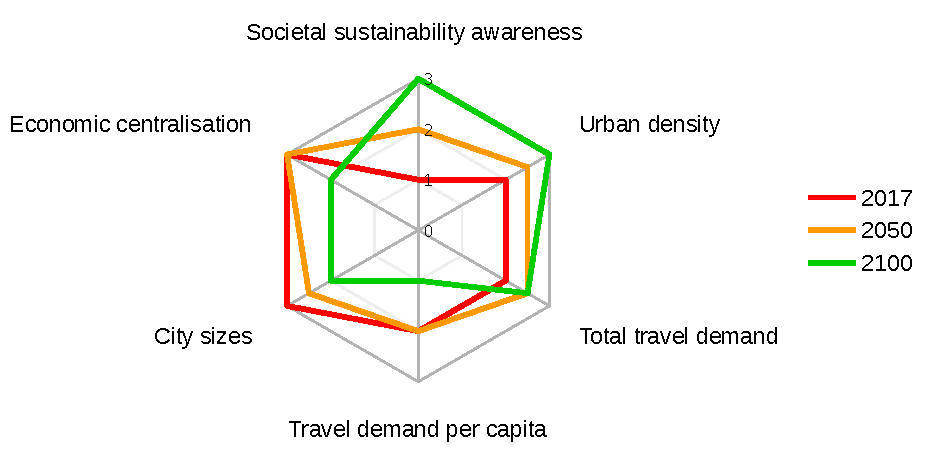
\includegraphics[width=0.8\textwidth]{figures/radar_development-scenario}
\caption[Shifts in development and land-use patterns in SSP1-MOB.]{Radar graph showing the shifts in development trends and land-use patterns found in SSP1 and SSP1-MOB for the years 2100, 2050 and 2017 (baseline). The following values are given to the qualitative variables: 3 for high, 2 for medium and 1 for low.}
\label{f:results:radar_development-scenario}
\end{figure}

\subsubsection*{Cultures of mobility}
As already highlighted in the \sref{ss:results:ssp1-mob-paradigm}, one of the key preconditions for the transition to a sustainable mobility paradigm is a change in the \emph{cultural perception} of mobility (how is it understood). The currently generalised notion of privately owning the means of transportation, namely automobiles, must be challenged if support for public transport is to grow. It is evident that such a challenge goes beyond the culture of mobility, into the general frame of material and ownership cultures. A reduced desire for both private ownership and private freedom of mobility ---which are in opposition to collective ownership and collective freedom--- would also pave the way for car sharing and carpooling schemes, which are currently deemed as lower-status, inconvenient alternatives. Therefore, it is the discourses around personal freedom and private property that must be radically challenged \parencite{zijlstra2012_SocioSpatialPerspective}.

Another key aspect of the mobility culture that must be challenged in the future is the conceptual link between movement and (again) the omnipresent discourse on freedom that forms the ideological core of the (neo)liberal society. The mental connection between freedom and freedom of movement must be broken if a reduction in travel demand is desired for the future of SSP1-MOB. The dissociation proves to be difficult, though, since the connection between freedom and mobility is strongly supported by the capitalist economic and ideological framework \parencite{freudendal-pedersen2009_MobilityDailyLife,sheller2012_EmergenceNewCultures}. However, the detachment of mobility from the general concept of freedom is promising from the sustainability point of view; if individual freedom is to emerge from other ``sources'' other than free movement, it is expected that the travel demand per capita gets lower. This is indeed related to the desired reduction of demand in SSP1-MOB, as portrayed in \fref{f:results:radar_development-scenario}.

Particularly, with regards to the most prevalent form of transportation nowadays, the automobile, a lot has to change in its perception from a cultural perspective. If the share of automobile demand has to drop so dramatically as portrayed in SSP1-MOB (from a dominant position to a niche-filing solution), a number of its cultural ``components'' \parencite{urry2004_SystemAutomobility} must be contested and changed:
%
\begin{enumerate}
\item Cars must not be conceived as technological marvels to be worshipped. Instead, they must be understood for what they are: tools for mobility.
\item A change in the value attributions to automobiles is necessary as well, in order to stop it being the second most item of individual consumption, after housing. Values such as freedom, safety, sexual drive or speed must be dissociated from automobiles.
\item Cultural discourses, imagery and symbolic status of automobiles as constituents of the ``good life'' must be contrasted with the impacts that it actually causes; they must be culturally subverted.
\item The subordination of other forms of mobility, such as slow modes, to automobility has to be contested. A new hierarchy of mobilities is needed for a future of denser, bigger and more compact urban areas.
\end{enumerate}

Finally, the shift of cultural perspective must happen not only at the user level, but also at the urban/traffic planner's. \textcite{banister2008_sustainablemobilityparadigm}, drawing from \textcite{marshall2001_challengesustainabletransport}, presents some of the foundation stones of the change to such a sustainable mobility planning paradigm:
%
\begin{enumerate}
\item Instead of speeding up traffic, slowing it down must be the new target for both users and planners.
\item Streets have to be seen as a space for urban life, rather than just public spaces occupied by private automobiles only.
\item Social and environmental multicriteria analyses regarding mobility need to be performed in addition to the already dominant (and only) economic assessments in urban planning.
\item Larger travel \emph{times} for similar or reduced travel \emph{distances} must become acceptable, in contrast to the current ever accelerating pace of society and mobility.
\item In general, attention has to shift from vehicles to people: human, personal mobility should be at the core of the frame, opposed to purely vehicle mobility.
\end{enumerate}

One last remark is worth to be discussed here, with regards to point 4 in the previous enumeration. An important and overseen aspect of sustainable mobility is the different conception of time. Drawing from the analysis that \textcite{zijlstra2012_SocioSpatialPerspective} make about cultural trends that support automobility, \emph{time} has played a central role in modern (capitalist) societies. The concept of time \emph{gaining} is so deeply embedded in modern cultures that acceleration, be it in production lines, communications, shopping activities or, relevantly, transport, has become a paradigmatic goal for almost any development effort in our society. Although not being explicit in the SSP1-MOB narrative, a change of mindset with respect to time is also desirable, since it would flatten the path for slow modes to take over. An example of such a change in lifestyles is already portrayed by \emph{slow cities} \parencite{mayer2006_SlowCitiesSustainable}.

\subsubsection*{Travel mode shifts}
One of the key aspects of the path to SSP1-MOB is travel mode shifting. This is, the relative reduction or increase in the demand share of the various travel modes available until 2100. This shift is visually shown in \fref{f:results:travel-demand-shares}, where the desired shares for 2050 and 2100 are portrayed, in accordance to the estimates given by \textcite{vuuren2017_Energylanduse}.

With respect to the previously discussed components of the backcasted path, culture and land-use patterns are not the only means to achieve the kind of transport mode shift shown in \fref{f:results:travel-demand-shares}. Two more patterns of change are identified in the SSP1-MOB narrative that should enable faster mode shift rates:
%
\begin{enumerate}
\item Demand management should play a more central role in traffic/urban planning. Following the terminology by \textcite{goodwin2012_ProvidingRoadCapacity}, planning should evolve from a road-centered ``predict-and-provide''\footnote{\textcite{goodwin2012_ProvidingRoadCapacity} originally refers, specifically, to infrastructure (roads/urban) planning approaches.} approach to a truly multi-modal ``predict-and-manage'' perspective. Traffic calming, road and congestion pricing mechanisms, multi-modal demand modelling and public transport facilitating policies (through, e.g., subsidies) should become commonplace in the future, in order to gradually shift travel demand towards the more sustainable transport modes.
\item Intermodal travel must become a reality in the SSP1-MOB world: it is the most prominent way to reduce unsustainable car usage in long-distance trips settings. Automobility is predominant in this type of trips, due to the (perceived) inconvenience of public transport, high costs of non-integrated public transport networks and lack of proper travel information for the end user \parencite{riley2010_IntermodalPassengerTransport}. Therefore, public transport networks must become integrated at much larger scales, with affordable fares and, very importantly, technologies must be developed to convey the necessary information to the users.
\end{enumerate}
 %
\begin{figure}
		\centering
  \begin{subfigure}{0.8\textwidth}
    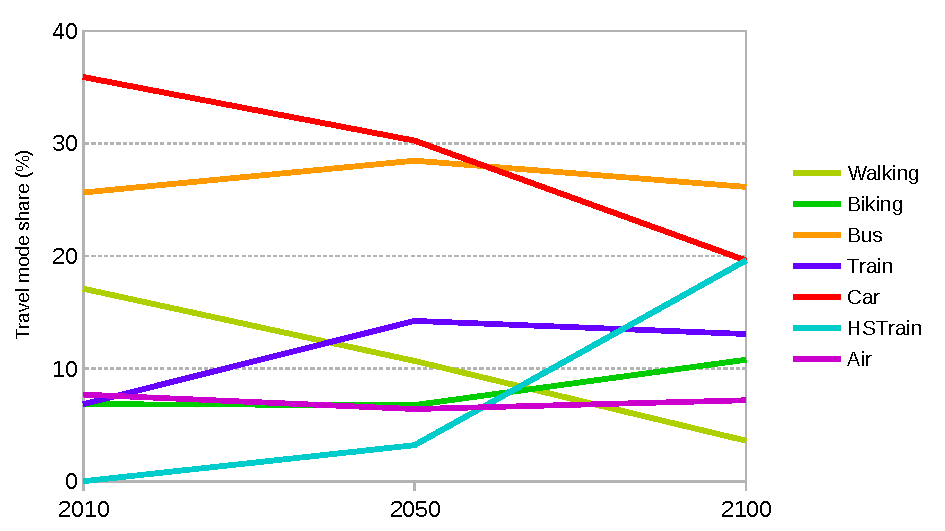
\includegraphics[width=\linewidth]{figures/line_travel-demand-shares.pdf}
    \caption{}
    \label{f:results:line_travel-demand-shares}
  \end{subfigure}
  \begin{subfigure}{0.8\textwidth}
    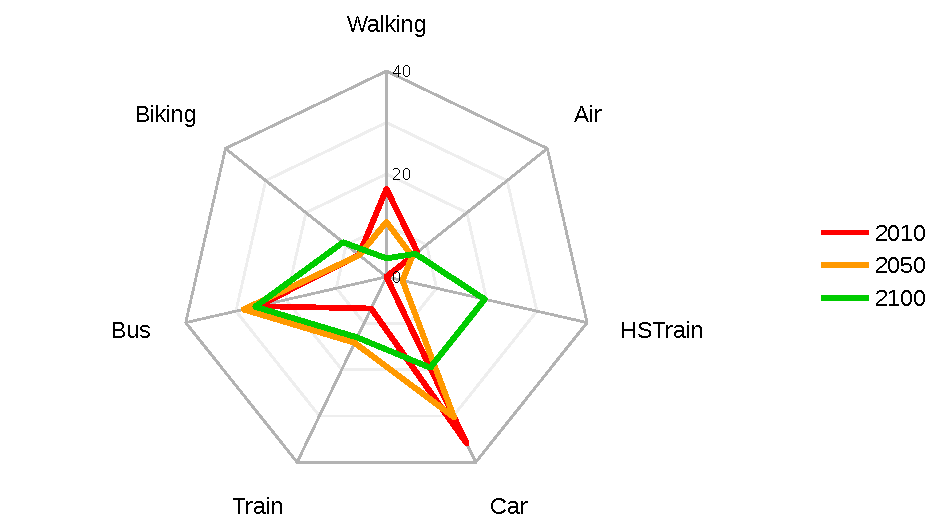
\includegraphics[width=\linewidth]{figures/radar_travel-demand-shares.pdf}
    \caption{}
    \label{f:results:radar_travel-demand-shares}
  \end{subfigure}
  \caption[Evolution and comparison of travel demand shares in SSP1-MOB.]{Evolution (a) and comparison (b) of total travel demand per transport mode (shares), in percentages, across the SSP1-MOB futures and the 2017 baseline. Note: the demand shares are approximated from the figures provided by \textcite{vuuren2017_Energylanduse} in their quantitative appraisal of the SSP1 scenario.}
  \label{f:results:travel-demand-shares}
\end{figure}

\subsubsection*{Vehicle and fuel technologies}
Finally, there is another key category of changes within the transport system that must be tackled in order to follow the path of SSP1-MOB: efficiency increases and technological progress. This applies mostly to the transport technologies themselves: vehicles must be made much more efficient if they are to be run on carbon-based fuels. An extensive electrification of the vehicles is also desired to reach not only low-carbon technologies, but also low-noise, low-emission vehicles that stop polluting the urban areas' air.

With regards to vehicle and fuel technologies, the SSP1-MOB narrative assumes the very high efficiency gains also assumed by \textcite{vuuren2017_Energylanduse} in their implementation of the SSP1 storyline. SSP1-MOB also draws from this implementation the higher share of renewable (bio)fuels in the transport sector and the emergence of hydrogen powered vehicles from 2050 onwards. Needless to say, these technological advances are linked to broader changes in the political and industrial arenas. A political will to devote resources into research and development of key technologies must be developed and, in turn, transport companies must embrace and push for a change in the technological bases of their products.

%%
%\begin{figure}
%		\centering
%  \begin{subfigure}{0.8\textwidth}
%    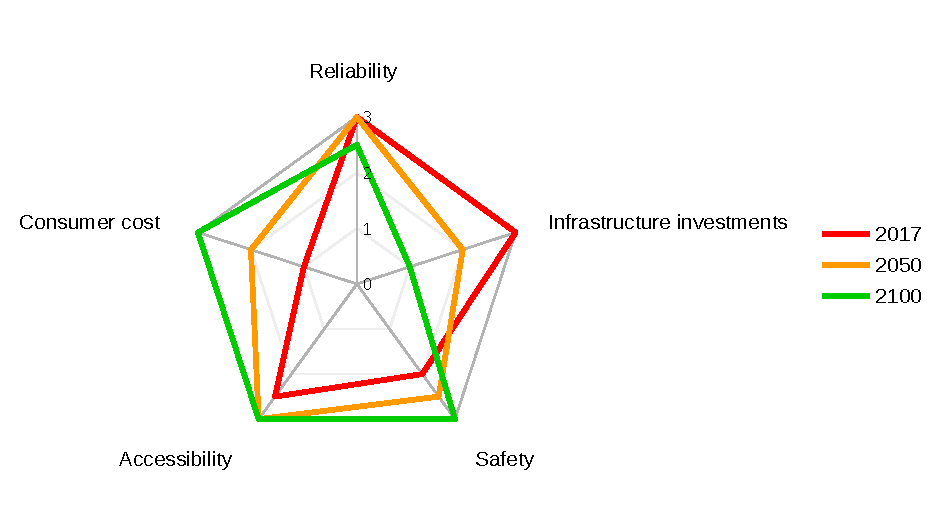
\includegraphics[width=\linewidth]{figures/radar_automobility.pdf}
%    \caption{}
%    \label{f:results:radar_automobility}
%  \end{subfigure}
%  \begin{subfigure}{0.8\textwidth}
%    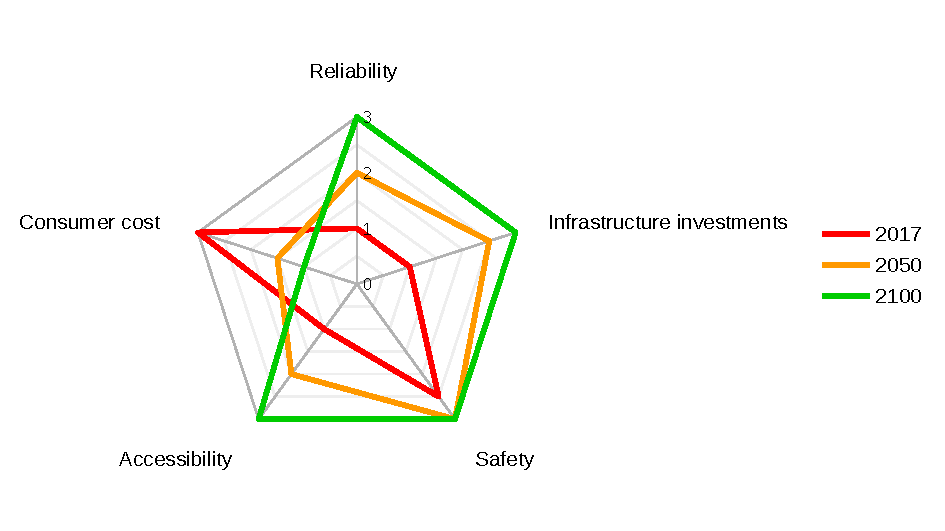
\includegraphics[width=\linewidth]{figures/radar_public-transport.pdf}
%    \caption{}
%    \label{f:results:radar_public-transport}
%  \end{subfigure}
%  \caption[]{}
%\end{figure}